\documentclass[10pt,a4paper]{article}
\usepackage[margin=1.65 cm,top=1.4 cm,bottom=1.5 cm]{geometry}
\usepackage[T1]{fontenc}
\usepackage[utf8]{inputenc}
\usepackage{lmodern,microtype,booktabs,tabularx,array,amsmath,graphicx,xcolor,colortbl,hyperref,enumitem,fancyhdr}
\usepackage{pgfplots}
\pgfplotsset{compat=1.18}
\definecolor{navy}{HTML}{183B56}\definecolor{teal}{HTML}{187F80}
\definecolor{orange}{HTML}{BE6E31}
\hypersetup{colorlinks=true,urlcolor=teal,linkcolor=navy,pdftitle={Thesis Progress Update: Routing Overhead and Post-Pruning Recovery},pdfauthor={Eren Olmez}}
\setlength{\parindent}{0 pt}\setlength{\parskip}{4 pt}\setlength{\emergencystretch}{2 em}
\renewcommand{\arraystretch}{1.12}
\setlist[itemize]{leftmargin=1.2 em,itemsep=1 pt,topsep=2 pt}
\pagestyle{fancy}\fancyhf{}\fancyhead[L]{\small\color{navy}Energy-efficient input-based model routing}
\fancyhead[R]{\small 6 November 2026}\fancyfoot[C]{\small\thepage}\setlength{\headheight}{13 pt}
\newcommand{\heading}[1]{\section*{\color{navy}#1}}
\newcommand{\smallcap}[1]{{\footnotesize\color{navy}#1}\par}
\pgfplotsset{meeting/.style={tick label style={font=\scriptsize},label style={font=\small},
  title style={font=\small},legend style={font=\scriptsize,draw=none,fill=none},
  grid=major,major grid style={draw=gray!18},axis line style={draw=gray!65},
  tick style={draw=gray!65},clip=false}}
\begin{document}
\begin{center}
{\Large\bfseries\color{navy}Thesis Progress Update}\\[3 pt]
{Eren Olmez}\\{6 November 2026}
\end{center}\vspace{-8 pt}
\heading{1. Batch scaling and router training cost}
This update follows the 29 October meeting: test the apparent batch-32 plateau, measure model residency and switching, reduce dispatch overhead, repeat router-energy measurements with warm-up, and test recovery after structural pruning. PC inference, Jetson estimates and the HPC classifier sweep are separate studies.

\textbf{Does inference stop improving beyond batch 32?}
The historical routed curve flattened or worsened above 32. In the controlled follow-up, each comparison held the FP16 engine, model, validation inputs and input/output boundary fixed. The original TensorRT optimization profile was retained. With input already on the GPU and output left on-device, both tested models improved from batch 32 to 128:

\begin{center}\small
\begin{tabular}{@{}lrrrrrr@{}}\toprule
 & & & \multicolumn{2}{c}{GPU-resident input} & \multicolumn{2}{c}{Host input to host logits}\\
\cmidrule(lr){4-5}\cmidrule(lr){6-7}
FP16 classifier & Batch & Test acc. & ms/image & GPU mJ/image & ms/image & GPU mJ/image\\
\midrule
ResNet101 & 32 & 85.85\% & 0.3355 & 23.170 & 0.3632 & 25.509\\
 & 64 & 85.85\% & 0.3265 & 23.162 & 0.3518 & 24.313\\
 & 128 & 85.85\% & 0.3190 & 22.125 & 0.3457 & 23.512\\
EfficientNet-B0 & 32 & 82.71\% & 0.1384 & 9.895 & 0.1701 & 12.140\\
 & 64 & 82.71\% & 0.1242 & 8.862 & 0.1548 & 11.354\\
 & 128 & 82.71\% & 0.1164 & 8.046 & 0.1456 & 10.497\\
\bottomrule\end{tabular}
\end{center}
\smallcap{Top-1 accuracy was measured separately on all 10,000 CIFAR-100 test images at each batch size. Neither FP16 engine changed any predicted class across the three batch sizes. Timing and energy come from 36 validation-input windows (three repeats per setting). Against batch 32, GPU-resident batch 128 cut latency/energy by 4.92\%/4.51\% for ResNet101 and 15.91\%/18.69\% for EfficientNet-B0. No timed thermal slowdown was sampled; power-cap flags remained.}

\textbf{What caused the historical plateau?}
No single cause was isolated. The historical audit found zero cache evictions at batches 32--128, so repeated reloads cannot explain that part of the curve. A separate routed diagnostic observed thermal slowdown and power-cap flags. Its first-sweep latency includes initial engine loads; repeated-sweep GPU energy amortizes those loads. These observations identify plausible contributors, not a proven cause of the historical curve.

\textbf{How does router fit cost compare with last week?} The October 29 measurements and this week's warmed fits each cover 20 TinyCNN training epochs. This week's timed fit used less GPU energy for seed 42 but more for seeds 45 and 48. Fit time followed the same pattern.
\begin{center}
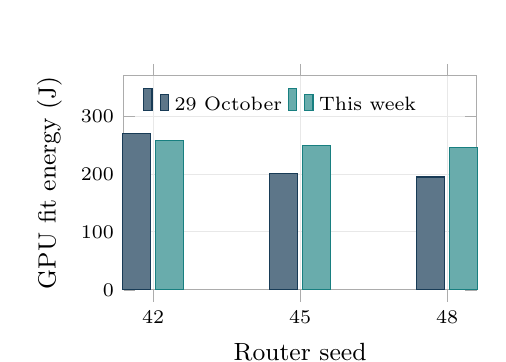
\begin{tikzpicture}
\begin{axis}[meeting,ybar,bar width=10pt,width=.50\linewidth,height=4.3cm,
 symbolic x coords={42,45,48},xtick=data,xlabel={Router seed},ylabel={GPU fit energy (J)},
 ymin=0,ymax=370,ytick={0,100,200,300},legend columns=2,legend pos=north west]
\addplot[fill=navy!70,draw=navy] coordinates {(42,270.437) (45,201.185) (48,195.008)};
\addplot[fill=teal!65,draw=teal] coordinates {(42,257.57) (45,248.65) (48,246.69)};
\legend{29 October,This week}
\end{axis}
\end{tikzpicture}\hfill
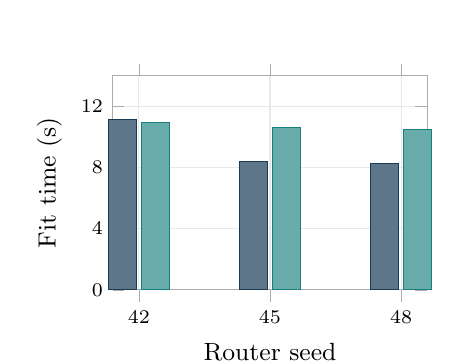
\begin{tikzpicture}
\begin{axis}[meeting,ybar,bar width=10pt,width=.46\linewidth,height=4.3cm,
 symbolic x coords={42,45,48},xtick=data,xlabel={Router seed},ylabel={Fit time (s)},
 ymin=0,ymax=14,ytick={0,4,8,12}]
\addplot[fill=navy!70,draw=navy] coordinates {(42,11.138) (45,8.389) (48,8.266)};
\addplot[fill=teal!65,draw=teal] coordinates {(42,10.934) (45,10.595) (48,10.463)};
\end{axis}
\end{tikzpicture}
\end{center}\vspace{-5pt}
\begin{center}\small
\begin{tabular}{@{}rrrrr@{}}\toprule
Seed & 29 Oct\ (s) & This week (s) & 29 Oct\ (GPU J) & This week (GPU J)\\
\midrule
42 & 11.138 & 10.934 & 270.437 & 257.57\\
45 & 8.389 & 10.595 & 201.185 & 248.65\\
48 & 8.266 & 10.463 & 195.008 & 246.69\\
\bottomrule\end{tabular}
\end{center}
\smallcap{One reported fit per seed on 29 October; medians of six fits per seed this week. This week's 100 dummy warm-up steps are outside the timed fit and cost energy themselves. These were separate sessions, so the differences do not isolate the effect of warm-up or replace last week's break-even estimates.}

\newpage
\heading{2. GPU residency and CPU--GPU dispatch}
\textbf{How many models can stay on the PC GPU?} On the RTX 2060, all retained TensorRT engines re-executed with their own contexts and buffers while keeping at least 1 GiB of VRAM free. Engine order matters:
\begin{center}\small
\begin{tabular}{@{}rrrr@{}}\toprule
Batch & Smallest engines first & Largest engines first & Architecture round-robin\\
\midrule
1 & 53 & 12 & 18\\
32 & 46 & 11 & 17\\
64 & 42 & 11 & 16\\
128 & 36 & 10 & 15\\
\bottomrule\end{tabular}
\end{center}
\smallcap{Demonstrated counts for these loading orders, not an absolute maximum or a test of holding all 213 configurations.}

\textbf{How often did the router switch models at batch 1?} With the same six classifiers available, three separately trained and calibrated TinyCNN routers (seeds 42, 45, and 48) switched on 3,936 (39.4\%), 5,010 (50.1\%), and 5,207 (52.1\%) of 9,999 consecutive image pairs, respectively. All saw the same 10,000 test images in different orders. The rates reflect both which models were chosen and the order of those choices, so they do not isolate the effect of training. A switch is a change in model choice, not a GPU reload.

\textbf{What is a CUDA Graph?} It records a sequence of GPU operations once so the CPU can submit the whole sequence for replay, instead of issuing the operations one by one. Here, after the CPU submits the replay, TinyCNN runs on the GPU and the GPU uses its scores to select and run just one of eight already-loaded classifiers. The control also runs inference on the GPU, but the CPU reads the routing scores and launches the selected classifier. Both paths made identical choices with no timed model reloads (seed 42).

\begin{center}
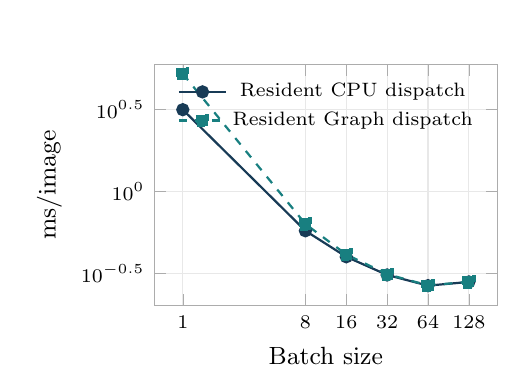
\begin{tikzpicture}
\begin{semilogyaxis}[meeting,width=.49\linewidth,height=4.65cm,xmode=log,log basis x=2,
 xtick={1,8,16,32,64,128},xticklabels={1,8,16,32,64,128},
 ylabel={ms/image},xlabel={Batch size},ymin=0.2,ymax=6,legend pos=north east]
\addplot[navy,thick,mark=*] coordinates {(1,3.1629) (8,0.5750) (16,0.3988) (32,0.3088) (64,0.2657) (128,0.2799)};
\addplot[teal,thick,mark=square*,dashed] coordinates {(1,5.2449) (8,0.6328) (16,0.4120) (32,0.3123) (64,0.2667) (128,0.2801)};
\legend{Resident CPU dispatch,Resident Graph dispatch}
\end{semilogyaxis}
\end{tikzpicture}\hfill
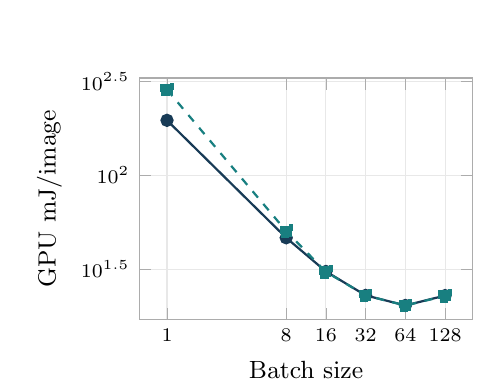
\begin{tikzpicture}
\begin{semilogyaxis}[meeting,width=.48\linewidth,height=4.65cm,xmode=log,log basis x=2,
 xtick={1,8,16,32,64,128},xticklabels={1,8,16,32,64,128},
 ylabel={GPU mJ/image},xlabel={Batch size},ymin=17,ymax=330]
\addplot[navy,thick,mark=*] coordinates {(1,196.350) (8,46.431) (16,30.711) (32,22.896) (64,20.237) (128,22.848)};
\addplot[teal,thick,mark=square*,dashed] coordinates {(1,286.124) (8,50.395) (16,30.546) (32,22.900) (64,20.213) (128,22.754)};
\end{semilogyaxis}
\end{tikzpicture}
\end{center}\vspace{-5pt}
\smallcap{Three-repeat medians on logarithmic axes. The eight-branch Graph worked correctly but did not make inference faster at any tested batch size. A separate two-model Graph saved 9.33\% latency and 11.33\% GPU energy; that result did not carry over to eight branches.}
\begin{center}\small
\setlength{\tabcolsep}{4.5pt}
\begin{tabular}{@{}rrrrrrrr@{}}\toprule
 & & \multicolumn{2}{c}{Latency (ms/image)} & \multicolumn{2}{c}{GPU energy (mJ/image)} & \multicolumn{2}{c}{Graph cost change}\\
\cmidrule(lr){3-4}\cmidrule(lr){5-6}\cmidrule(lr){7-8}
Batch & Val.\ acc. & CPU & Graph & CPU & Graph & Latency & Energy\\
\midrule
1 & 85.16\% & 3.163 & 5.245 & 196.35 & 286.12 & $+65.83$\% & $+45.72$\%\\
8 & 86.23\% & 0.575 & 0.633 & 46.43 & 50.40 & $+10.05$\% & $+8.54$\%\\
16 & 86.04\% & 0.399 & 0.412 & 30.71 & 30.55 & $+3.31$\% & $-0.54$\%\\
32 & 85.74\% & 0.309 & 0.312 & 22.90 & 22.90 & $+1.13$\% & $+0.02$\%\\
64 & 85.06\% & 0.266 & 0.267 & 20.24 & 20.21 & $+0.39$\% & $-0.12$\%\\
128 & 85.35\% & 0.280 & 0.280 & 22.85 & 22.75 & $+0.07$\% & $-0.41$\%\\
\bottomrule\end{tabular}
\end{center}
\smallcap{Positive means more time or energy than CPU dispatch; percentages use unrounded medians. At batch 1, Graph took about 66\% longer and used about 46\% more GPU energy. At batches 16--128 the energy differences were below 1\%. Predictions matched on all 1,024 calibration images.}

\textbf{Jetson Orin Nano 8 GB estimate.} With a 3 GiB OS allowance and 1.5$\times$ PC allocation multiplier, the model predicts 24/3/9 engines for the same three order types, or about 11,001 FP32 128px tensors in a separate two-classifier-plus-router scenario. Models and images compete for shared memory. These are PC-based estimates, not measured Jetson capacity, latency or energy.

\newpage
\heading{3. Fresh structural pruning and Adam fine-tuning}
\textbf{What did one epoch recover?} Both Adam rates started from the same freshly pruned ResNet18 p30 weights. The unpruned 128px checkpoint scored 79.16\% and the freshly pruned model 1.00\% on the original 5,000-image validation split. Requested p30 removed 50.40\% of parameters and 58.12\% of MACs.

\begin{center}\small
\begin{tabular}{@{}lrrl@{}}\toprule
Adam learning rate & Epoch 1 validation & Epoch 5 validation & Best extended result\\
\midrule
0.01 & 34.70\% & 58.38\% & Not extended\\
0.001 & 58.10\% & 68.90\% & 72.74\% (epoch 17)\\
\bottomrule\end{tabular}
\end{center}
At 0.001 the pilot stopped at epoch 22, five epochs after its last qualifying improvement. One epoch exceeded the historical p30 SGD validation reference (55.66\%), but additional epochs recovered another 14.64 percentage points. This is not a matched Adam-versus-SGD optimizer ablation. On the official test set, this p30 checkpoint scored 71.82\% overall: motorcycle, orchid, and sunflower tied for best (93\%), and seal was worst (36\%).

\textbf{Does the recovery extend across pruning levels?} All nine ResNet18 levels are complete in the new PC campaign. The plot shows the two sets of checkpoints on the original classifier validation split. The unpruned reference makes clear how much accuracy is left unrecovered at each pruning level.

\begin{center}
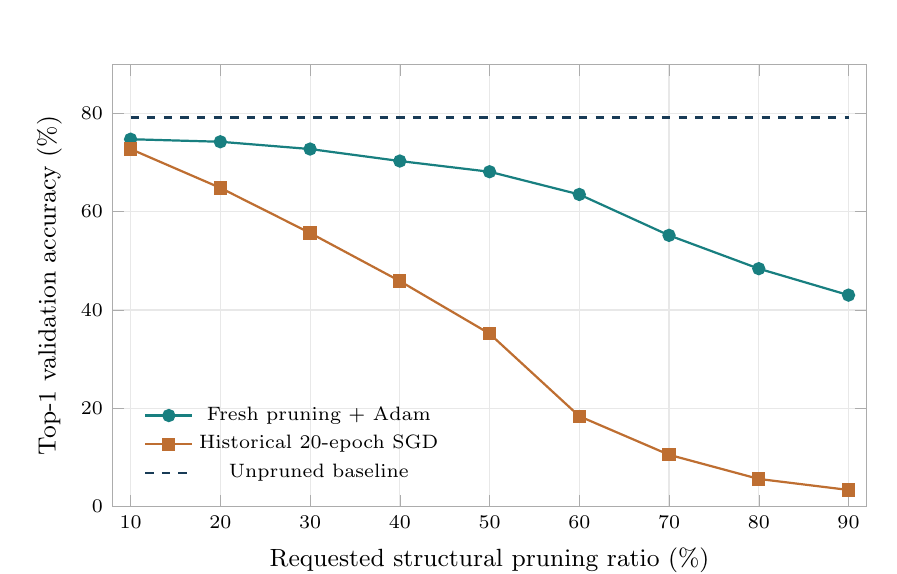
\begin{tikzpicture}
\begin{axis}[meeting,width=.92\linewidth,height=7.2cm,xlabel={Requested structural pruning ratio (\%)},
 ylabel={Top-1 validation accuracy (\%)},xmin=8,xmax=92,ymin=0,ymax=90,
 xtick={10,20,30,40,50,60,70,80,90},ytick={0,20,40,60,80},legend pos=south west]
\addplot[teal,thick,mark=*] coordinates {(10,74.74) (20,74.22) (30,72.74) (40,70.30) (50,68.12) (60,63.50) (70,55.18) (80,48.40) (90,43.02)};
\addplot[orange,thick,mark=square*] coordinates {(10,72.74) (20,64.84) (30,55.66) (40,45.88) (50,35.18) (60,18.38) (70,10.54) (80,5.62) (90,3.38)};
\addplot[navy,thick,dashed] coordinates {(10,79.16) (90,79.16)};
\legend{Fresh pruning + Adam,Historical 20-epoch SGD,Unpruned baseline}
\end{axis}
\end{tikzpicture}
\end{center}\vspace{-5pt}
\smallcap{Validation, not test accuracy. Requested pruning ratio is not the actual parameter or MAC reduction. The two recovery protocols differ; the separation is descriptive and not an isolated optimizer effect.}
\begin{center}\small
\begin{tabular}{@{}lrrrrrrrrr@{}}\toprule
Requested ratio (\%) & 10 & 20 & 30 & 40 & 50 & 60 & 70 & 80 & 90\\\midrule
Adam val.\ (\%) & 74.74 & 74.22 & 72.74 & 70.30 & 68.12 & 63.50 & 55.18 & 48.40 & 43.02\\
SGD val.\ (\%) & 72.74 & 64.84 & 55.66 & 45.88 & 35.18 & 18.38 & 10.54 & 5.62 & 3.38\\
\bottomrule\end{tabular}
\end{center}

\textbf{Fine-tuning is complete; benchmarking is separate.} All 63 checkpoints were verified (27 trained on PC, 36 on HPC): seven architectures at nine pruning levels each. Each run started from the original trained weights before pruning and used Adam at 0.001. Checkpoints were selected on validation, not test. All 63 have been exported to ONNX for benchmarking; that does not yet establish a latency or energy result.

\textbf{How many images repay router training energy?}
\begin{center}\small
\renewcommand{\arraystretch}{1.23}
\begin{tabularx}{.64\linewidth}{>{\centering\arraybackslash}p{.24\linewidth}>{\raggedleft\arraybackslash}X}
\toprule
\rowcolor{navy!9}\textbf{Batch size} & \textbf{Images to break even}\\\midrule
1 & 2,399\\
\rowcolor{navy!4}8 & \textemdash\\
16 & 9,348\\
\rowcolor{navy!4}32 & 3,440\\
64 & 3,277\\
\rowcolor{navy!4}128 & 3,333\\\bottomrule
\end{tabularx}
\end{center}
\smallcap{GPU energy only, without an accuracy filter. Baseline: always run unpruned ResNet101 FP32. The dash means no break-even point: at batch 8, routing used more energy per image. October 29 measurements; batch 1 used six resident models.}

\newpage
\heading{4. HPC training progress}
\textbf{HPC training from scratch.} This sweep is separate from the fine-tuning bank. W\&B recorded 353/1,728 completed runs (20.43\%) and 71,277/345,600 epochs (20.62\%). All four runs marked running had fresh metrics; 11 were marked failed or crashed. These counts do not verify Slurm state or checkpoints.

\begin{center}\small
\begin{tabular}{@{}lrrrrr@{}}\toprule
Active architecture (case) & Epoch & Latest val. acc. & Val. loss & Run-best val. acc. & Historical FP32 val.\\\midrule
ResNet50 (362) & 183 & 79.26\% & 0.796 & 79.90\% & 83.94\%\\
ResNet101 (363) & 110 & 74.26\% & 0.974 & 77.60\% & 85.88\%\\
EfficientNet-B0 (366) & 124 & 64.70\% & 1.331 & 64.76\% & 83.14\%\\
ShuffleNetV2 (367) & 71 & 47.58\% & 1.930 & 53.38\% & 75.72\%\\\bottomrule
\end{tabular}
\end{center}
\smallcap{Each run is planned for 200 epochs. Run-best is the highest validation accuracy observed so far in that run. The table below reports the highest observed validation accuracy across all runs of each architecture.}

\textbf{What is varied?} Eight architectures, with 72 recipes each. Each recipe combines one optimizer with its allowed initial learning rate and weight decay, one learning-rate schedule, and CutMix on or off. All runs are planned for 200 epochs without early stopping.
\begin{center}\small
\begin{tabular}{@{}lll@{}}\toprule
Optimizer & Initial learning rates & Weight decay\\\midrule
SGD & 0.03, 0.1, 0.2 & 0.0001, 0.0005\\
Adam & 0.0003, 0.001, 0.003 & 0.0001, 0.0005\\
AdamW & 0.0003, 0.001, 0.003 & 0.01, 0.05\\\bottomrule
\end{tabular}
\end{center}
\smallcap{Schedule: cosine or divide the rate by 10 at epochs 80 and 120. CutMix: off or $\alpha=1$ (mixes patches and labels between training images). Each recipe is repeated to measure variability.}

\begin{center}\small
\begin{tabular}{@{}lrrrr@{}}\toprule
Architecture & Best validation (case) & Initial LR & Weight decay & Historical FP32 val.\\
\midrule
ResNet18 & 80.12\% (312) & 0.1 & 0.0005 & 79.16\%\\
ResNet34 & 81.66\% (329) & 0.1 & 0.0005 & 82.98\%\\
ResNet50 & 81.26\% (314) & 0.1 & 0.0005 & 83.94\%\\
ResNet101 & 81.82\% (139) & 0.03 & 0.0005 & 85.88\%\\
MobileNetV3 Small & 64.42\% (228) & 0.1 & 0.0001 & 61.82\%\\
MobileNetV3 Large & 72.52\% (237) & 0.1 & 0.0001 & 82.04\%\\
EfficientNet-B0 & 72.70\% (142) & 0.03 & 0.0005 & 83.14\%\\
ShuffleNetV2 $\times$1.0 & 75.48\% (127) & 0.03 & 0.0005 & 75.72\%\\
\bottomrule\end{tabular}
\end{center}
\smallcap{Best observed validation is a single-run maximum, not a recipe ranking. All eight rows currently come from completed SGD runs with cosine scheduling and CutMix on. Current models train from random initialization at 32px. Historical unpruned TensorRT FP32 used ImageNet initialization, 128px inputs and a different validation split.}

\textbf{Next.} Measure the new fine-tuned bank on PC at batches 1/8/16/32/64/128 with matched fixed-model and unpruned references. Use the same host-input-to-prediction boundary for each method and report ms/image and GPU mJ/image alongside the historical results. Continue auditing the separate HPC sweep.
\newpage
\heading{5. Which classes are easiest and hardest after pruning?}
We evaluated all 63 frozen fine-tuned checkpoints on the \textbf{official CIFAR-100 test set}: 10,000 images, 100 per class. Inference used PyTorch FP32 at 128px. The first table shows one checkpoint per architecture, chosen before evaluating the test set (10\% requested pruning for all seven). Both heatmaps cover all nine pruning levels. Every accuracy on this page is test accuracy.
\begin{center}\small
\begin{tabularx}{\linewidth}{@{}lrrXX@{}}\toprule
Architecture & Pruning & Overall & Worst class & Best class(es) \\ \midrule
ResNet18 & 10\% & 75.07\% & boy (41\%) & skyscraper (97\%) \\
ResNet34 & 10\% & 75.50\% & shrew (40\%) & motorcycle / mountain (+1 ties) (95\%) \\
ResNet50 & 10\% & 76.02\% & girl (36\%) & motorcycle (97\%) \\
ResNet101 & 10\% & 76.08\% & seal (43\%) & orange (96\%) \\
MobileNetV3 Small & 10\% & 60.32\% & girl / otter (23\%) & motorcycle / wardrobe (90\%) \\
MobileNetV3 Large & 10\% & 71.33\% & woman (37\%) & orange / road (95\%) \\
EfficientNet-B0 & 10\% & 71.22\% & seal (40\%) & motorcycle (96\%) \\
\bottomrule\end{tabularx}
\end{center}
\textbf{How does the weakest class change as pruning increases?}
\begin{center}\small\setlength{\tabcolsep}{4.2pt}
\begin{tabular}{@{}lrrrrrrrrr@{}}\toprule
Requested pruning (\%) & 10 & 20 & 30 & 40 & 50 & 60 & 70 & 80 & 90 \\ \midrule
ResNet18 & \cellcolor{teal!26}41 & \cellcolor{teal!21}33 & \cellcolor{teal!23}36 & \cellcolor{teal!24}38 & \cellcolor{teal!19}30 & \cellcolor{teal!11}17 & \cellcolor{teal!8}13 & \cellcolor{teal!1}3 & \cellcolor{teal!0}1 \\
ResNet34 & \cellcolor{teal!26}40 & \cellcolor{teal!29}45 & \cellcolor{teal!18}28 & \cellcolor{teal!27}43 & \cellcolor{teal!16}25 & \cellcolor{teal!18}29 & \cellcolor{teal!6}10 & \cellcolor{teal!3}5 & \cellcolor{teal!2}4 \\
ResNet50 & \cellcolor{teal!23}36 & \cellcolor{teal!25}39 & \cellcolor{teal!27}42 & \cellcolor{teal!26}40 & \cellcolor{teal!29}45 & \cellcolor{teal!15}24 & \cellcolor{teal!18}29 & \cellcolor{teal!3}6 & \cellcolor{teal!1}3 \\
ResNet101 & \cellcolor{teal!27}43 & \cellcolor{teal!25}39 & \cellcolor{teal!24}37 & \cellcolor{teal!24}38 & \cellcolor{teal!19}30 & \cellcolor{teal!10}16 & \cellcolor{teal!3}6 & \cellcolor{teal!1}3 & \cellcolor{teal!1}2 \\
MobileNetV3 Small & \cellcolor{teal!14}23 & \cellcolor{teal!11}18 & \cellcolor{teal!13}21 & \cellcolor{teal!15}24 & \cellcolor{teal!14}22 & \cellcolor{teal!10}16 & \cellcolor{teal!11}17 & \cellcolor{teal!5}8 & \cellcolor{teal!2}4 \\
MobileNetV3 Large & \cellcolor{teal!24}37 & \cellcolor{teal!20}32 & \cellcolor{teal!17}27 & \cellcolor{teal!14}23 & \cellcolor{teal!18}29 & \cellcolor{teal!15}24 & \cellcolor{teal!16}26 & \cellcolor{teal!8}13 & \cellcolor{teal!3}6 \\
EfficientNet-B0 & \cellcolor{teal!26}40 & \cellcolor{teal!11}18 & \cellcolor{teal!14}23 & \cellcolor{teal!22}35 & \cellcolor{teal!16}26 & \cellcolor{teal!11}17 & \cellcolor{teal!15}24 & \cellcolor{teal!9}15 & \cellcolor{teal!5}8 \\
\bottomrule\end{tabular}
\end{center}
\smallcap{Each cell is the lowest class accuracy (\%) at that pruning level; darker means higher accuracy. The weakest class can change from cell to cell.}
\textbf{How does the strongest class change as pruning increases?}
\begin{center}\small\setlength{\tabcolsep}{4.2pt}
\begin{tabular}{@{}lrrrrrrrrr@{}}\toprule
Requested pruning (\%) & 10 & 20 & 30 & 40 & 50 & 60 & 70 & 80 & 90 \\ \midrule
ResNet18 & \cellcolor{teal!63}97 & \cellcolor{teal!61}95 & \cellcolor{teal!60}93 & \cellcolor{teal!62}96 & \cellcolor{teal!61}94 & \cellcolor{teal!59}91 & \cellcolor{teal!59}91 & \cellcolor{teal!55}86 & \cellcolor{teal!53}82 \\
ResNet34 & \cellcolor{teal!61}95 & \cellcolor{teal!63}97 & \cellcolor{teal!62}96 & \cellcolor{teal!61}94 & \cellcolor{teal!61}95 & \cellcolor{teal!62}96 & \cellcolor{teal!59}92 & \cellcolor{teal!57}89 & \cellcolor{teal!57}88 \\
ResNet50 & \cellcolor{teal!63}97 & \cellcolor{teal!63}97 & \cellcolor{teal!62}96 & \cellcolor{teal!62}96 & \cellcolor{teal!62}96 & \cellcolor{teal!61}95 & \cellcolor{teal!61}95 & \cellcolor{teal!58}90 & \cellcolor{teal!57}89 \\
ResNet101 & \cellcolor{teal!62}96 & \cellcolor{teal!61}95 & \cellcolor{teal!63}98 & \cellcolor{teal!62}96 & \cellcolor{teal!63}98 & \cellcolor{teal!62}96 & \cellcolor{teal!56}87 & \cellcolor{teal!55}86 & \cellcolor{teal!50}78 \\
MobileNetV3 Small & \cellcolor{teal!58}90 & \cellcolor{teal!58}90 & \cellcolor{teal!57}89 & \cellcolor{teal!59}92 & \cellcolor{teal!57}89 & \cellcolor{teal!55}86 & \cellcolor{teal!56}87 & \cellcolor{teal!56}87 & \cellcolor{teal!53}82 \\
MobileNetV3 Large & \cellcolor{teal!61}95 & \cellcolor{teal!61}94 & \cellcolor{teal!60}93 & \cellcolor{teal!59}91 & \cellcolor{teal!61}94 & \cellcolor{teal!61}94 & \cellcolor{teal!57}89 & \cellcolor{teal!57}89 & \cellcolor{teal!58}90 \\
EfficientNet-B0 & \cellcolor{teal!62}96 & \cellcolor{teal!62}96 & \cellcolor{teal!61}94 & \cellcolor{teal!61}94 & \cellcolor{teal!59}92 & \cellcolor{teal!60}93 & \cellcolor{teal!57}89 & \cellcolor{teal!61}94 & \cellcolor{teal!57}89 \\
\bottomrule\end{tabular}
\end{center}
\smallcap{Each cell is the highest class accuracy (\%) at that pruning level, using the same color scale as above. The strongest class can change from cell to cell.}
\textbf{Where do models disagree most on class accuracy?} At each selected pruning level, this is the class with the largest accuracy gap between models.
\begin{center}\small\begin{tabularx}{\linewidth}{@{}rlXX@{}}\toprule
Pruning & Class & Highest accuracy & Lowest accuracy \\ \midrule
10\% & man & ResNet101 (76\%) & MobileNetV3 Small (31\%) \\
50\% & leopard & ResNet50 (82\%) & MobileNetV3 Small (44\%) \\
90\% & orange & ResNet50 (89\%) & ResNet34 (42\%) \\
\bottomrule\end{tabularx}\end{center}

\smallcap{Test results were not used to train or choose checkpoints. Differences in class accuracy suggest where models might complement one another, but do not establish a routing gain.}
\end{document}
